\chapter{总结}
\section{项目中遇到的问题及解决方法}
<<<<<<< HEAD

=======
\subsection{Feign报错}
在项目开发过程中,经常会抛出~IllegalStateException~异常,经过思考和查阅资料,我们发现这是因为在~Feign~中,我们使用了~@RequestParam~注解,而~Feign~不支持解析~@RequestParam~注解,所以我们需要使用要用~value~标明对应的参数。

\subsection{ScanMapper报错}
在开发项目后端时,我们最开始使用了~@MapperScan~注解,而在~MyBatis~中,~@MapperScan~注解需要指定对应的包路径。然而,由于有时后项目无法识别已有的XML资源,导致我们的项目在负载均衡场景下出现了问题,经常发生报错而自动刷新,随后又重新恢复。后来我们发现,可以在~application.yml~文件中配置~mybatis.mapper-locations~属性,指定对应的XML资源路径,这样就可以解决这个问题。
而最终呈现的代码版本去掉了~@MapperScan~注解,改用配置文件的方式指定XML资源路径,解决了这个问题。

\subsection{请求绕过网关直接访问微服务}
在进行项目测试时,我们发现到在发出请求时可以直接绕过网关访问微服务,导致网关的负载均衡、熔断以及 token 认证功能都会直接失效。为了解决这个问题,我们让网关每次发送请求时,给请求添加一个from请求头,微服务端收到请求时会先查看是否有该请求头以判断请求是否是通过网关转发,如果不是会返回错误。
>>>>>>> 53eb9252 (完善报告结构)

\section{项目开发过程}
\subsection{项目共享仓库}
我们对于本实践项目使用 GITHUB 进行仓库共享,让每一名组员可以在该仓库上进行代码的修改以及同步,大幅度增加实践效率。通过以下网址,可以游览到本项目的共享仓库页面:https://github.com/stainsatin/elm
\begin{figure}[htbp]
    \centering
    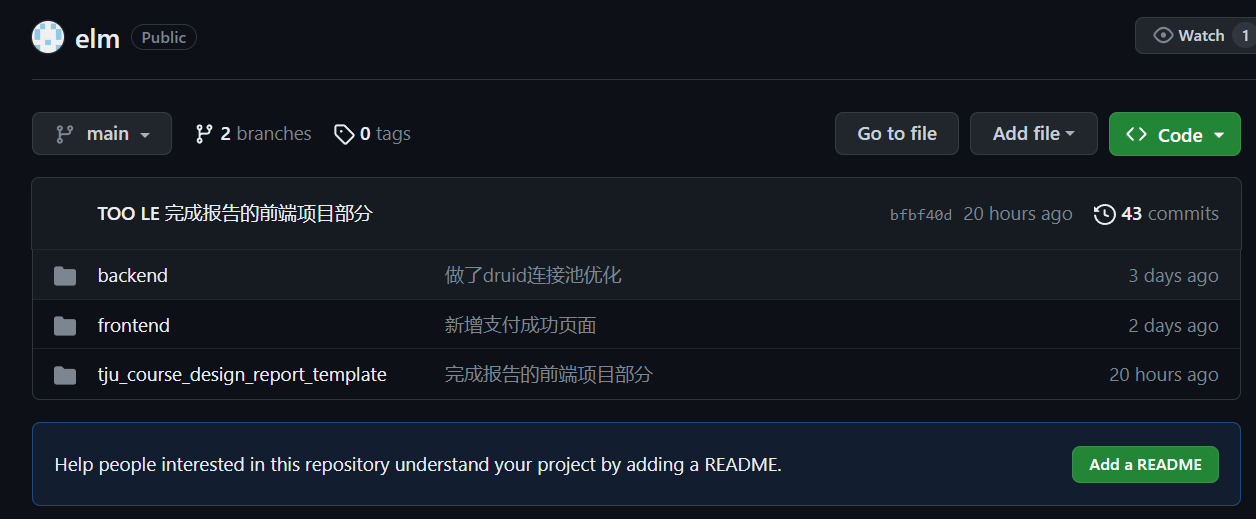
\includegraphics[width=0.8\textwidth]{githubmain.png}
    \caption{GITHUB 共享仓库页面}\label{fig:githubmain}
    \vspace{\baselineskip}
\end{figure}

本次实践项目的共享仓库于 4 月 4 日创建,仓库里的成员包括我们每一名组员。如上图~\ref{fig:githubmain}~所示,仓库里的内容包括本次实践项目的前端、后端与实践报告的目录,并且我们每一名组员都在此共享仓库上进行了多次代码的复制和提交。经过接近一个月的项目开发,以下是我们的共享仓库数据视图,如图~\ref{fig:commit}~至图所示:

\begin{figure}[htbp]
    \centering
    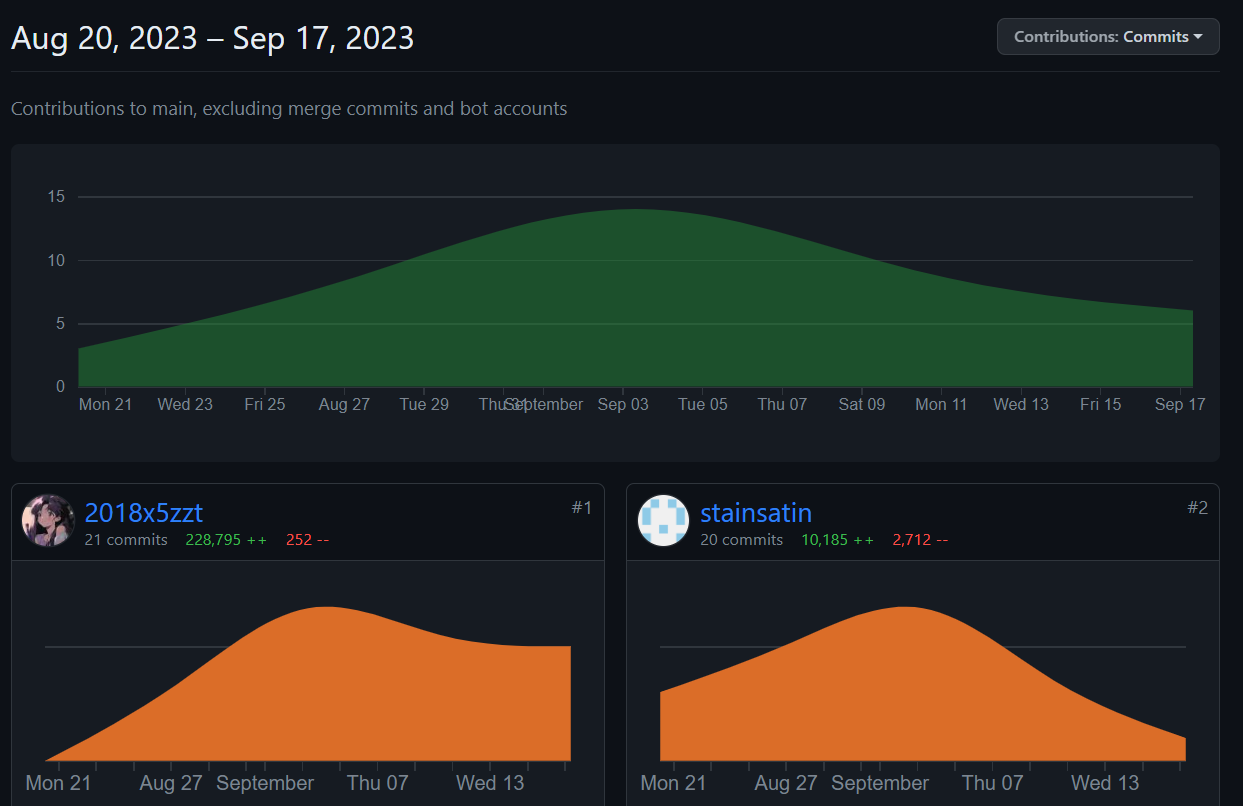
\includegraphics[width=0.7\textwidth]{commit}
    \caption{GITHUB 共享仓库提交视图}\label{fig:commit}
    \vspace{\baselineskip}
\end{figure}
\begin{figure}[htbp]
    \centering
    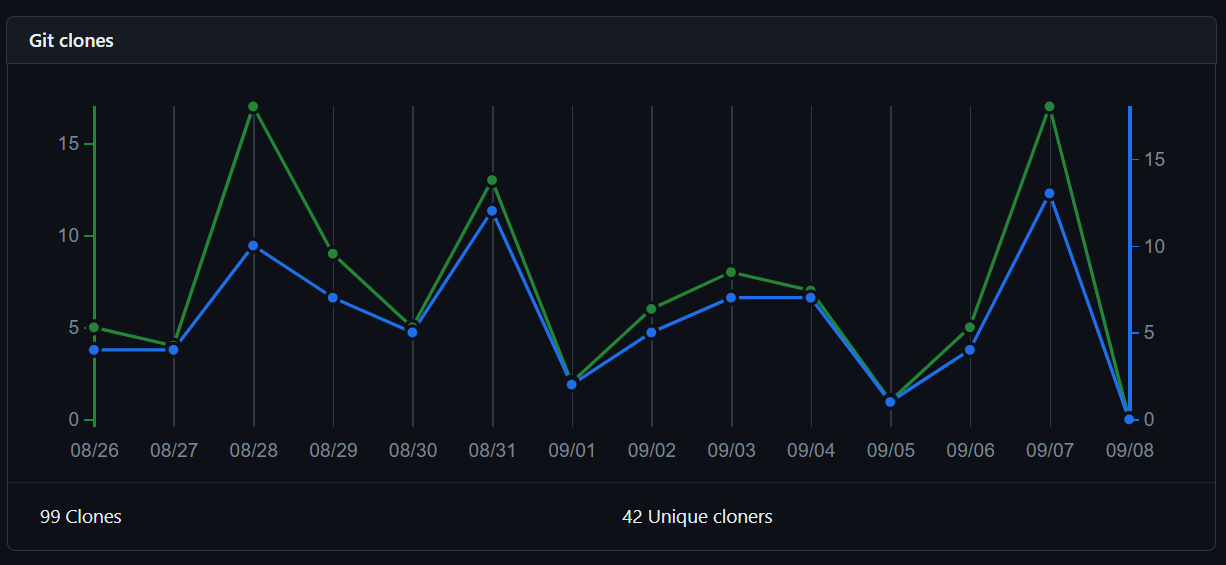
\includegraphics[width=0.8\textwidth]{clone}
    \caption{GITHUB 共享仓库复制视图}\label{fig:clone}
    \vspace{\baselineskip}
\end{figure}
\begin{figure}[htbp]
    \centering
    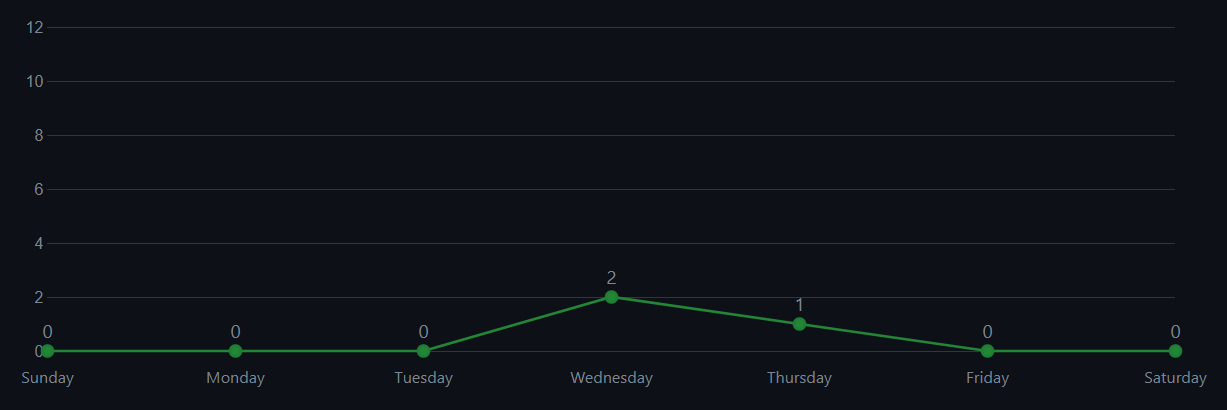
\includegraphics[width=0.8\textwidth]{week1commit}
    \caption{GITHUB 共享仓库第一周提交次数视图}\label{fig:week1commit}
    \vspace{\baselineskip}
\end{figure}
\begin{figure}[htbp]
    \centering
    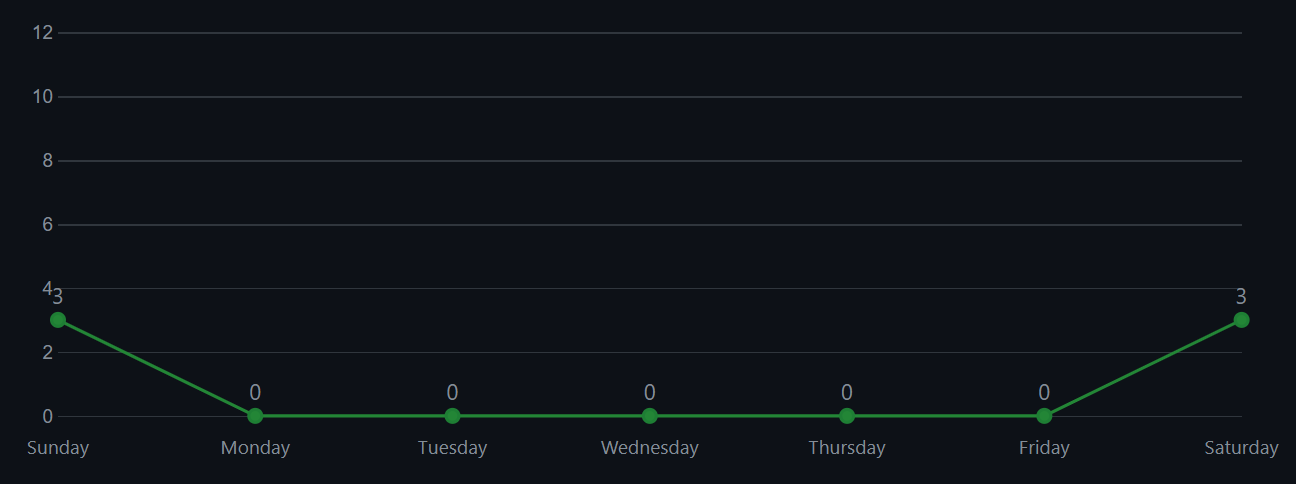
\includegraphics[width=0.8\textwidth]{week2commit}
    \caption{GITHUB 共享仓库第二周提交次数视图}\label{fig:week2commit}
    \vspace{\baselineskip}
\end{figure}
\begin{figure}[htbp]
    \centering
    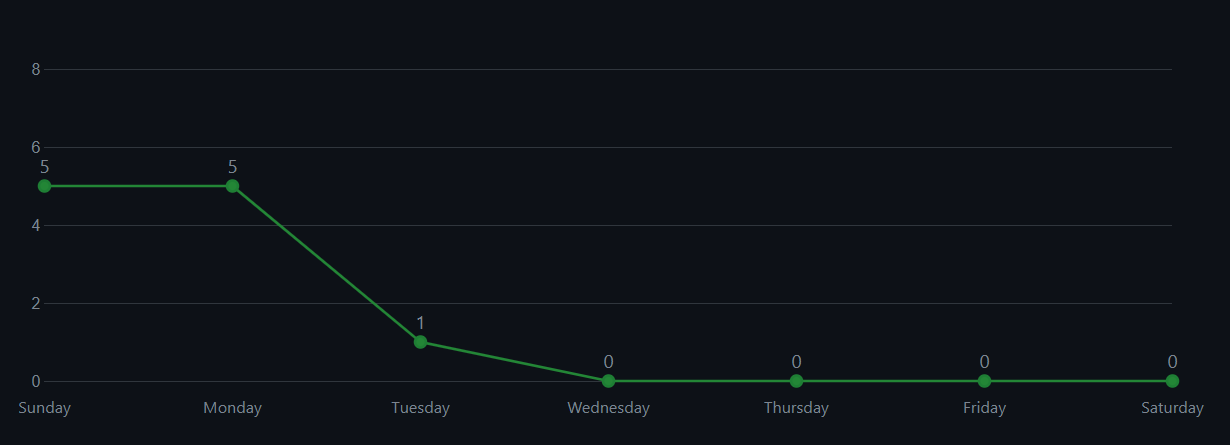
\includegraphics[width=0.8\textwidth]{week3commit}
    \caption{GITHUB 共享仓库第三周提交次数视图}\label{fig:week3commit}
    \vspace{\baselineskip}
\end{figure}
\begin{figure}[htbp]
    \centering
    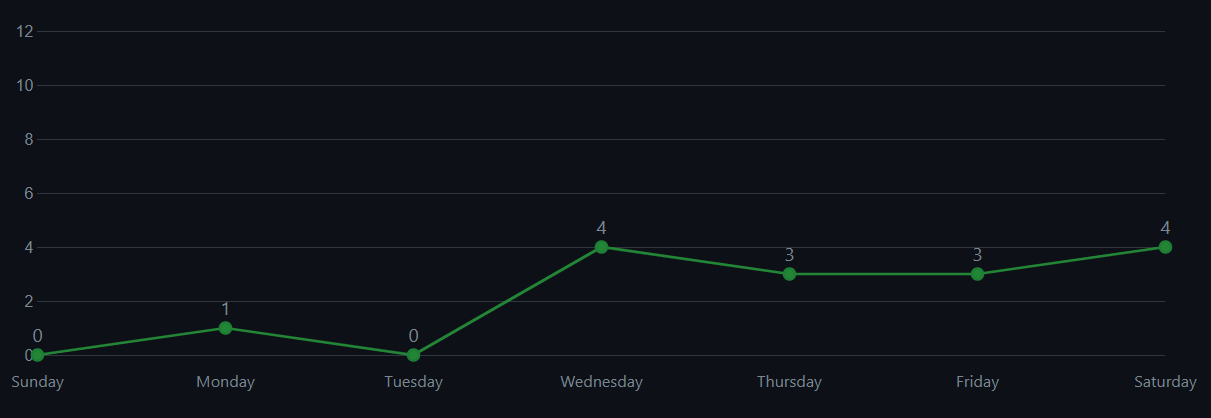
\includegraphics[width=0.8\textwidth]{week4commit}
    \caption{GITHUB 共享仓库第四周提交次数视图}\label{fig:week4commit}
    \vspace{\baselineskip}
\end{figure}
\begin{figure}[htbp]
    \centering
    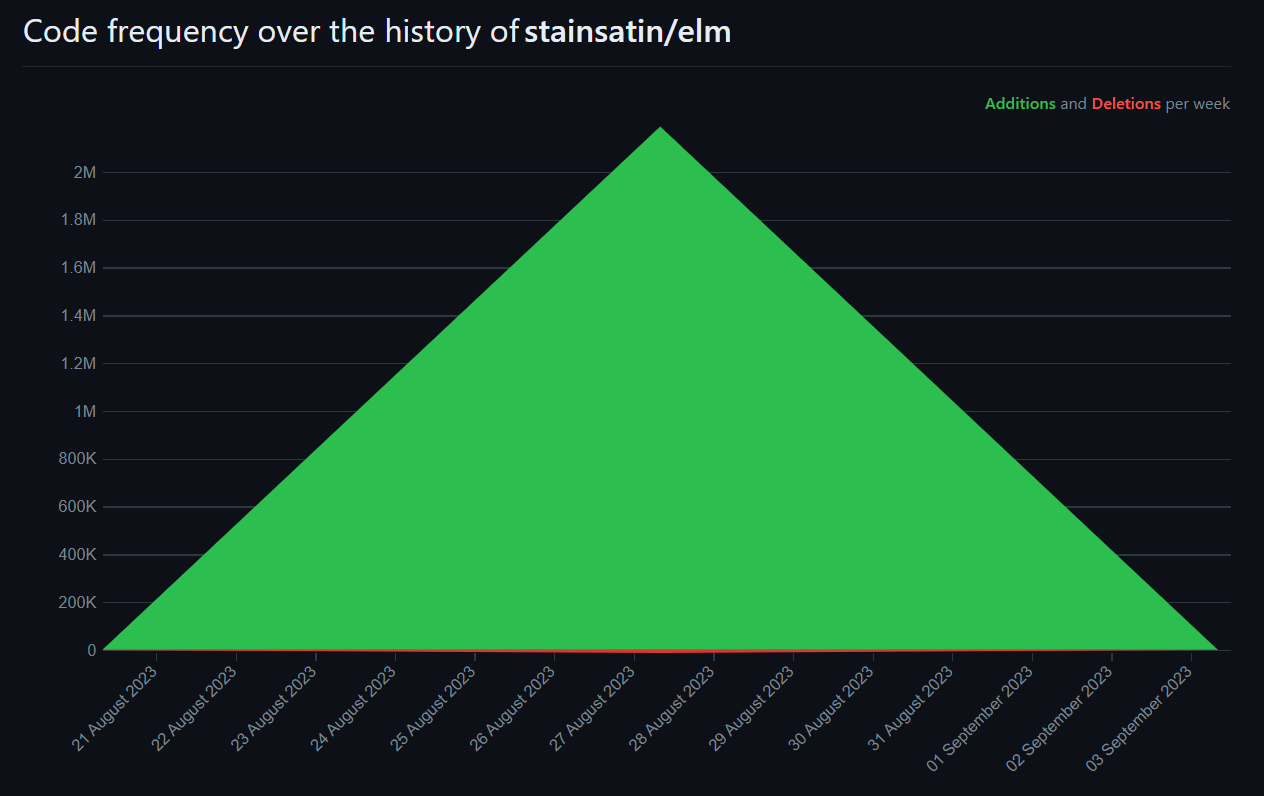
\includegraphics[width=0.7\textwidth]{codefrequency}
    \caption{GITHUB 共享仓库代码频率视图}\label{fig:codefrequency}
    \vspace{\baselineskip}
\end{figure}

\section{开发总结}
总的来说,这是一个比较复杂的软件项目,其中涉及到了 Spring Cloud 框架、Vue3 等一系列网页开发的技术。在这样的情况下,我们四位小组成员分工明确,可以较为顺利且相互配合地完成自身的开发部分。在交互,测试的过程中,我们遇到了各种各样的问题,这些问题我们也能够准确找到问题出现的地方,知道这部分问题是由谁负责完成。大家积极配合彼此工作,才能让项目比较顺利的进行下去。

在整个项目开发过程中,每个成员都做出了重要的贡献。大家分工明确,对自己所做的部分认真负责,同时在某些阶段,当部分组员任务较重时,大家也会主动去分担任务缓解彼此压力。我们每个人都发挥自己所长,为项目做出贡献。

总的来说,这是一次收获颇丰的实践经历。通过这次对程序设计高级实践的学习,我们学会的很多网页开发的技术,项目管理的经验,也锻炼了在面对复杂问题,出现意外情况时钻研思考,独立解决问题的能力。另外我们也培养了团队成员间积极沟通,配合,团结协作的能力。相信这次宝贵的经验能让我们运用在后续在软件工程专业的学习过程中。

